\chapter{Reference management}
\label{sec:literature}

For typesetting our first thesis in \LaTeX{}, the last core functionality to learn is citing literature.
Our references are gathered in a bibliography file.
Once we reference one of its entries from our \LaTeX{} document, Bib\TeX{} (a 
program similar to the standard \sh{pdflatex} compiler)
can insert automatically generated citations.
It will format them in a bibliography style of our choice.

\section{The bibliography file}
Our \textbf{bibliography collection} consists of multiple literature entries in a pre-defined format, such that they can be processed by Bib\TeX{}.
An exemplary item can be seen in \cref{lst:bibfile-sample-entry}.

\begin{figure}[H]
  \codeblock{bibtex}{listings/literature/bibliography-entry.bib}

  \caption{Exemplary bibliography entry}
  \label{lst:bibfile-sample-entry}
\end{figure}

The type of the bibliography entry is specified after the opening \mono{@} sign (article, book, proceedings, …).
What follows is a list of important attributes like title and author.
Whether they are required or not depends on the type of the entry.
In any case, we will need the first entry after the opening braces: the Bib\TeX{} key.
This is the identifier that we will use to reference the entry in our \LaTeX{} document.
Bib\TeX{} keys can be chosen freely, but have to be unique.
Typically, they will consist of a combination of authors, publication dates, and topics.\newpage

\textbf{Bibliography files} can be compiled manually, yet it is more common to use programs like JabRef,\footnote{Cf. \url{https://www.jabref.org/}.} Zotero\footnote{Cf. \url{https://www.zotero.org/}.} or the widely-used software Citavi\footnote{Vgl. \url{https://www.citavi.com/de}.}.
While JabRef operates directly on your bibliography file, Zotero and Citavi projects\footnote{Vgl. \url{https://www1.citavi.com/sub/manual5/de/exporting_to_bibtex.html}.} can be exported to bibliography files to use them in \LaTeX{} documents.

\textbf{Bibliography entries} are provided by many academic search engines, including Google Scholar (cf. \cref{fig:google-scholar-bibtex}).
When using them, make sure that the entries are cohesive across your reference collection and complete with regard to their attributes.
A high-quality (although, unfortunately, incomplete) source for Bib\TeX{} entries is the dblp computer science bibliography.\footnote{Available at \url{https://dblp.org/search}.}

\begin{figure}[H]
  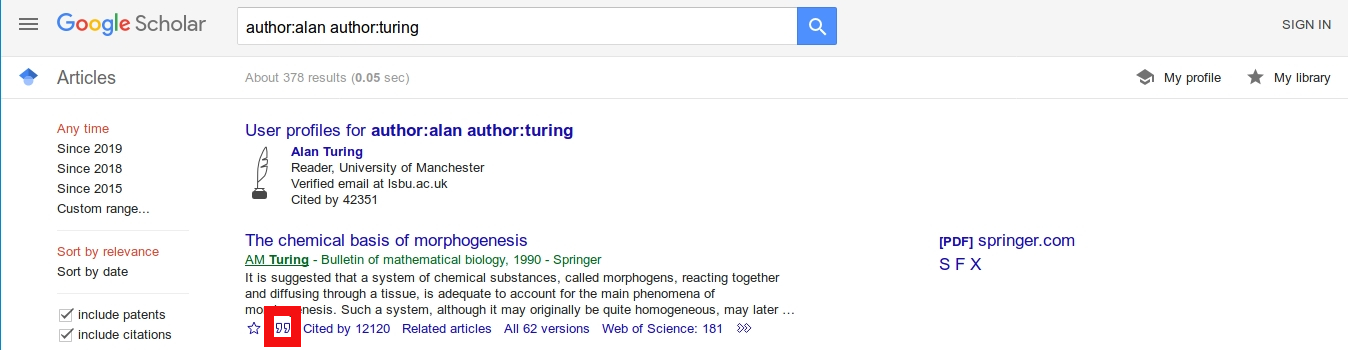
\includegraphics[width=\textwidth]{graphics/google_bibtex1.jpg}  
  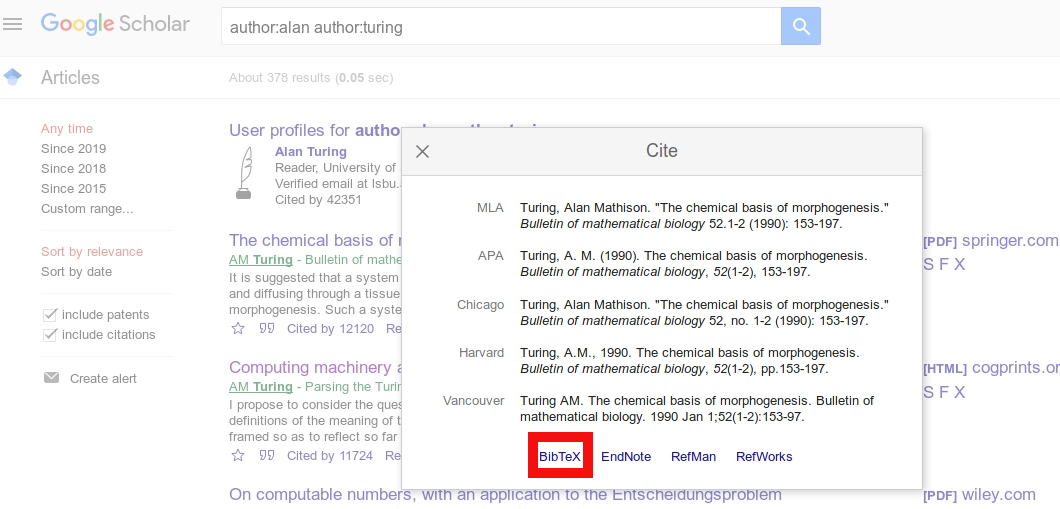
\includegraphics[width=\textwidth]{graphics/google_bibtex2.jpg}  
  \caption{Loading Bib\TeX{} entries from Google Scholar}
  \label{fig:google-scholar-bibtex}
\end{figure}

\section{Citing}
Bib\TeX{} extends \LaTeX{} by several commands (cf. \cref{tbl:bibtex-commands}). 
Make sure to include the \pkg{natbib} package for this purpose.

\begin{table}[H]
  \centering
  \begin{tabular}{ll}
  \toprule
  Function                 & Command \\ \midrule
  Citing authors           & \code{latex}{\textbackslash citeauthor\{<source>\}} \\
  Citing sources           & \code{latex}{\textbackslash cite\{<source>\}} \\
  Citing pages             & \code{latex}{\textbackslash cite[p. 15]\{<source>\}} \\
  Custom citations         & \code{latex}{\textbackslash cite[<prefix>][<suffix>]\{<source>\}} \\
  Including the bibliography     & \code{latex}{\textbackslash bibliography\{<bibliographyfile>\}} \\
  Setting the bibliography style & \code{latex}{\textbackslash bibliographystyle\{<style>\}} \\ \bottomrule
  \end{tabular}
  \caption{Commands for citations}
  \label{tbl:bibtex-commands}
\end{table}

The \code{latex}{<source>} of a citation is always a Bib\TeX key.
The list of available citation styles\footnote{Head to Overleaf for a rather complete list: \url{https://www.overleaf.com/learn/latex/Biblatex_citation_styles}} includes \mono{alpha}, \mono{natdin}, and \mono{apa}.
The table of references will always appear where the \code{latex}{\textbackslash bibliography\{…\}} command was put.
The \code{latex}{\textbackslash cite} command comes with many variants.\footnote{cf. \url{https://www.economics.utoronto.ca/osborne/latex/BIBTEX.HTM}}

\Example{lst:natdin-example}{literature/natdin-example}{literature/natdin-example_bib}{Exemplary citations in the \mono{natdin} style.}
